\section{Verification}
The exact meaning of verification is confusing \cite{thomas_arts}. The
definition may differ in comparison of academic or industrial use. Even in
different phases of the safety life cycle verification is conducted in various
forms \cite[8:9.2]{ISO26262}.

\subsection{Formal Verification}
%Skriv n�got luddigt
Formal verification is very hard to achieve for software, due to the state space
explosion problem. To achieve formal verification, one must visit every state
that exists, and prove for each of those states, that the code is correct. State
space explosion occur when a small increase of elements rapidly raises the
number of combinations to a computational maximum. %% SKRIV OM!!!!!!!!!!!

\subsection{Semi formal verification}
%Skriv n�got �n mer luddigt

\section{Industrial Standards} It is useful to distinguish between
systems with different levels of dependability, and determine where the hazards
exists\cite{COURSEBOOK:safety-critical}. When this risk analysis is completed
%% �verv�g kommatecken mellan dessa satser
and appropriate reliability and availability requirements is assigned to the
system, the system can be identified by a certain safety integrity level (SIL).
If this number is high, the system will experience a more rigorous design and
testing than could be justified for a lesser demanding system. These levels is
more defined in standards IEC~61508 and ISO~26262.

%\setion{Functional Safety}
% Kanske n�got vi vill skriva om? N�ms i metoden

\subsection {IEC~61508 and ISO~26262}

%G�r skillnad p� verifikation och verifikation. Dvs vilken fas handlar det om?
Automotive software for safety related systems is required to be designed,
implemented and verified by the standard ISO~26262, which handles functional
safety for automotive equipment. For a higher level of integrity ISO~26262
strongly recommends that semi formal verification of each module should be
executed \cite[Part 6]{ISO26262}.  It also recommends a formal verification, but
because of the state-space complexity this is hard to achieve.

ISO~26262 is built on IEC~61508 which is titled Functional Safety of
Electrical/Electronic/Programmable Electronic Safety-related Systems. IEC~61508
can be applied to any kind of industry while ISO~26262 is defined only for the
automotive industry. IEC~61508 have four safety integrity levels (SIL) ranked
1-4. SIL 4 is the highest and should be applied where a failure can
do devastating damage to a large area. %% �r det inte ocks� s� att om det �r
%% ganska farligt men riskerar att h�nda ofta s� ska den ocks� klassas som SIL 4.
The automotive industry is improbable to have this risk. That is why ISO~26262
%% "that is why" - syftar p� att detta �r huvudanledningen. det �r nog m�nga
%% olika anledningar att ISO26262 har utvecklats.
exists which also defines four levels of SIL called automotive safety integrity
level (ASIL). The ASIL range from A-D, where D is the highest and roughly
translate to SIL 3.

\subsection{AUTOSAR (AUTomotive Open System ARchitecture)}
%Beskriv vad fan det �r
%K�lla http://www.autosar.org/
The AUTOSAR platform has a layered software architecture. This means that the
architecture is divided to a number of different layers, such as the application
layer, runtime environment, the basic software layer, and the
microcontroller. In the Figure~\ref{FIG:AUTOSAR:architecture} the basic software
layer is represented as four different parts; services, ECU
abstraction, microcontroller abstraction, and complex drivers.

\begin{figure}[!ht]
  \begin{center}
    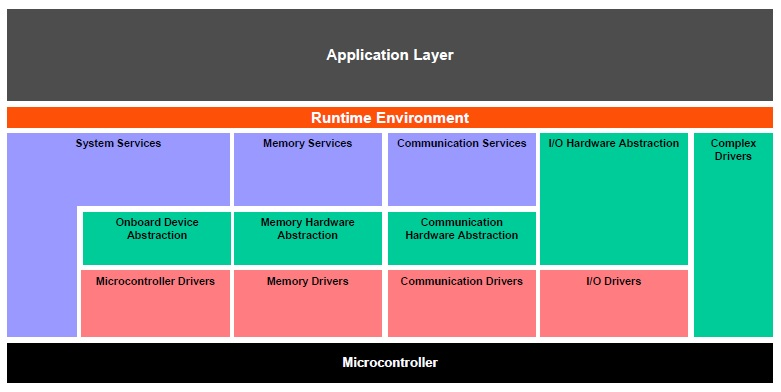
\includegraphics[keepaspectratio, width=\linewidth]{pictures/autosar_architecture.jpg}
  \end{center}
  \caption{The AUTOSAR software architecture. Noticeable is that the basic
    software layer is divided further into three categories with more subsections.}
  \label{FIG:AUTOSAR:architecture}
\end{figure}

The runtime environment is the OS, and the microcontroller is the hardware. The
software running in the application layer is applications such as sensors and
actuators. %% skriva n�got mer om applikationslagret.

%% Saxxat fr�n AUTOSAR Layered software
% Automotive ECUs have the properties: strong interaction with hardware,
% connection to vehicle networks, limited computing power and memory, real time
% system, program execution from internal or external flash memory.

% The AUTOSAR architecture is a generic approach, standard modules can have
% extended functionality and still be compliant.

One example of how the different parts in the basic software layer is
integrated, is the watchdog, which consist of several parts as seen in Figure~\ref{FIG:AUTOSAR:watchdog}. The
microcontroller abstraction layer has the drivers for the watchdog, the
interaction with the microcontroller. Then there is the watchdog interface at
the ECU abstraction layer. The watchdog interface is the onboard device
abstraction. Last is the watchdog manager which runs as a system service in the
service layer.

\begin{figure}[!ht]
  \begin{center}
    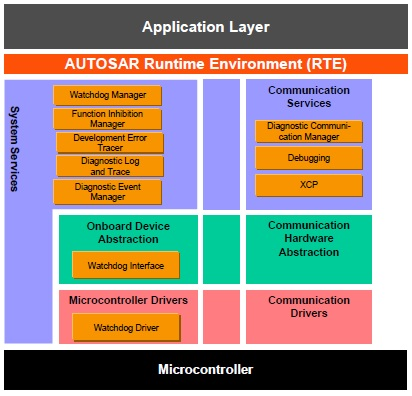
\includegraphics{pictures/watchdog_architecture.jpg}
  \end{center}
  \caption{The Watchdog and some other related modules.}
  \label{FIG:AUTOSAR:watchdog}
\end{figure}

The watchdog have a number of dependencies to other services in the basic
software layer. For example when an error is found by the watchdog, it should be
reported to either the diagnostic event manager or the development error
tracer. Two services used for error management. %% bra eller anus att skriva av
                                %% den ska skicka fel till DEM eller DET n�r vi
                                %% skriver i n�sta avsnitt att det g�r att ta
                                %% bort DEM rapporteringen?

AUTOSARs concept is to make it possible for vehicle manufacturers to buy modules
from different software developers, which will still work together in
unison. For vehicle manufacturers to have different work done by the same
software developer's
module, the standard introduce configurations. There exist a number of variables
to configure. In the watchdog manager, there is for example variables that
specify if the watchdog manager should report errors to the diagnostic event
manager (DEM), or which type of supervision that should be done and what to
supervise.


% Some of the specifications in AUTOSAR is left quite open for interpretation.
% %% beskriv varf�r dessa inte �r tillr�ckligt definierade, och varf�r olika
% %% konfigurationer existerar.
% This makes it possible for vehicle developers to have different specifications
% for a configuration. Some parts of those configuration specifications is
% generated into code, while other is manually written or added as a configurable.

\section{Existing Software}
There are a number of existing software tools whose aim are to simplify the
implementation of verification and testing.
%% ..och helt pl�tsligt presenteras en lista av n�got..
\begin{itemize}
\item QuickCheck
\item SPIN
\item McErlang
\item $\mu$CRL toolset
\item CADP
\item Parasoft C/C++test
%\item Erlang and QuickCheck
%\item Symlink
%\item CORE
%\item Isabelle
\end{itemize}

\subsection{QuickCheck}
QuickCheck was invented be Koen Claessen and John Hughes, as a testing module
for Haskell, in 2000.
In 2006 John Hughes founded the Company Quviq together with
Thomas Arts. Quviq offers a commercial version of QuickCheck for Erlang.
The main difference, except from the programming paradigms, is that
the commercial version of QuickCheck has a C-testing interface. Hence it
possible to test C-code in Erlang with help of QuickCheck. All code for tests
is written in Erlang and checked against API calls to the C-code. It is actually
not necessary to have actual source code; it is enough to only have compiled library
files.

QuickCheck tests a program with specification implemented as properties that
the program must hold \cite{QUICKCHECK:manual}. QuickCheck has guided random
test generation, this means that the samples can be weighted to cover certain
parts of the state-space with more likelihood.

%% Erlang �r inget verktyg per se. vi borde skriva om det, men passar det in
%% h�r?
\subsection{Erlang}
Erlang can easily communicate with other programming language by
using byte streams. There have been some work done including Erlang,
AUTOSAR and QuickCheck, mostly by the QuviQ company\cite{QUVIQ:flyer}.
%% "mostly"? skriva n�got om Volvo och SP ocks�?
Imperative coding requires state based testing(?). QuviQ have developed a library in
Erlang for this purpose(?).

% \subsection{CORE}
% A specification package developed by British Aerospace and System Designers.

%\subsection{Promela}

\subsection{SPIN}
SPIN is used to trace logical design errors in distributed
software\cite{SPIN:manual}. It supports a high level language, Promela, to
specify system descriptions. Promela is an acronym for PROcess MEta LAnguage, and
is a verification model language. The system properties that should be checked
are written in logical temporal language (LTL), and SPIN reports errors such as
deadlocks, race conditions and incompleteness between these properties and the
system model. It also supports embedded C code as part of the model
specifications. It supports random, interactive and guided simulation, with both
partial and exhaustive proof techniques.

\subsection{McErlang}
McErlang is a model checker written in Erlang used for verifying distributed
Erlang programs\cite{MCERLANG:model-checker}. Its purpose is to check a program
against a correctness property, but can also among other things check safety
or liveness properties.

McErlang offers two depth-first state traversal model checking algorithms; one
checks safety properties and the other is used for checking the liveness
properties. McErlang also implements weak process fairness, by omitting non-fair
loops from the accepting runs in its liveness algorithm.

%% jag tror mcerlang ing�r i QuickCheck suiten. den blir installerad tillsammans
%% med QuickCheck iaf.

\subsection{$\mu$CRL toolset} $\mu$CRL is a process algebraic language which is
suited for the analysis of distributed systems. The toolkit is built on this
language and contains a theorem prover based on binary decision
diagrams\cite{MCRL:manual}.

\subsection{CADP} Construction and Analysis of Distributed Processes (CADP),
formerly CAESAR/ALDEBARAN Development Package, is a toolset for the design of
distributed systems\cite{CADP:manual}. It includes, among others, tools for
equivalence checking, state-space manipulation and model checking, and it also
includes several verification algorithms. It provides functionality as
step-by-step simulation to parallel model checking.

\subsection{Parasoft C++test}
Parasoft C++ is a commercial software with a huge range of functionality,
developed by the Parasoft company, with the purpose of testing software written
in C or C++. Parasoft claims that it should be possible to satisfy ASIL
requirements using their software(?).
%\subsection{Isabelle}
% Isabelle theorem prover is an interactive theorem prover, successor of the
% Higher Order Logic (HOL) theorem prover

\section{Verification Methods}
The standard IEC~61508 propose two methods to say that a program is formal
verified. The key is to model the program into one of the following machines.

\begin{enumerate}
\item \label{enum:FSM} Finite state machines/state transition diagrams
\item Time Petri nets
\end{enumerate}

IEC~61508 emphasises that Time Petri nets are best suited for concurrent
programs. Regarding method \ref{enum:FSM} the following criteria needs to be
satisfied for the implemented state machine to be formal verified:

\begin{description}
\item[completeness] the system must have an action and new state for every input
in every state,
\item[consistency] only one state change is described for each state/input
pair, and
\item[reachability] whether or not it is possible to get from one state to
another by any sequence of inputs.
\end{description}

If the state machine is correctly implemented it exist a correct model of the
%% det �r n�got konstigt med denna meningen men jag kan inte riktigt s�tta
%% fingret p� det.
%% kan vara att: om SM �r korrekt implementerad - s� �r originalprogrammet
%% formellt verifierat. �r detta verkligen allt som kr�vs?
original program, then the original program is formal verified.

Since most program specification are written in natural languages there may be
lots of ambiguities. Consequently a lot of techniques has been developed to reduce
such cases. These techniques are often referred to as semi formal verification,
because they lack of mathematical rigour associated with formal
verification. These methods use textual, graphical or other notation; often
several techniques are used in unity. % These tests may not be

The description of semi formal verification in IEC~61508 states: \\
''Semi-formal methods provide a means of developing a description of a system at
some stage in its development, i.e. specification, design or coding. The
description can in some cases be analysed by machine or animated to display
various aspects of the system behaviour.''
